\chapter{Interface} \label{chapter4}

In this chapter, we will be discussing the presentation layer of the proposed solution of this paper. We will present the design conventions and strategies, the timetable widget, and the new elements and flows. 

We will focus on the User Interface (UI) elements and how they are interconnected and behave, defining the User Experience (UX).

\section{Design conventions and strategies} \label{5:conv}

As the application is cross-platform, it was primarily designed to behave the same on all devices. However, as Android and iOS applications are conceptually different, ACS UPB Mobile borrows design conventions from both environments \cite{apple2020human} and delivers a coherent interface and experience.
As we previously mentioned, widgets play an essential part in the interface. As the Skia engine renders them, we are guaranteed that the user flows remain the same, while the composing graphical elements might differ. These differences are related to the operating system primitives called upon when building a page or a widget, and be can, for example, the top bar, pop-ups, and alerts.

The primary elements that we will use will be Cards\footnote{https://api.flutter.dev/flutter/material/Card-class.html} and Lists\footnote{https://flutter.dev/docs/cookbook/lists/mixed-list}. They are already heavily used inside the application, versatile enough to contain various children elements, and interactive to respond to user input. 
\clearpage

The pages that we will update or add are : 
~

Homepage: 
\begin{itemize}
            \setlength{\topsep}{0.5pt}
            \setlength{\itemsep}{0.5pt}
            \setlength{\parsep}{0.5pt}
            \item A new Card that displays pieces of information about upcoming events.
            \item A new Card for the Planner feature that displays information about the following tasks: it also doubles as the entry point for the  Planner page.
\end{itemize}

~

Timetable: 
\begin{itemize}
            \setlength{\topsep}{0.5pt}
            \setlength{\itemsep}{0.5pt}
            \setlength{\parsep}{0.5pt}
            \item A Gantt diagram \cite{wilson2003gantt} way of displaying tasks.
\end{itemize}

~

Add/Edit task event: 
\begin{itemize}
            \setlength{\topsep}{0.5pt}
            \setlength{\itemsep}{0.5pt}
            \setlength{\parsep}{0.5pt}
            \item Add new options for adding tasks, with relevant fields.
\end{itemize}

~

Class: 
\begin{itemize}
            \setlength{\topsep}{0.5pt}
            \setlength{\itemsep}{0.5pt}
            \setlength{\parsep}{0.5pt}
            \item A new card to show all the events.
\end{itemize}

~

Event Instance: 
\begin{itemize}
            \setlength{\topsep}{0.5pt}
            \setlength{\itemsep}{0.5pt}
            \setlength{\parsep}{0.5pt}
            \item Button to hide/unhide event.
            \item List tiles for task-specific fields.
            \item Button to add/edit the goal.
            \item Cards for each element of the goal.
\end{itemize}

~

Planner Page: 
\begin{itemize}
            \setlength{\topsep}{0.5pt}
            \setlength{\itemsep}{0.5pt}
            \setlength{\parsep}{0.5pt}
            \item An effort graph.
            \item Lists for current, hidden, and past events.
            
\end{itemize}

\clearpage

\section{Timetable} \label{5:timetable}

The timetable is based upon the public package: timetable: 0.2.9 \footnote{https://pub.dev/packages/timetable}, which is another open-source project created by a student \footnote{https://github.com/JonasWanke} from Hasso-Plattner-Institute \footnote{https://hpi.de/}, a university in Potsdam, Germany.

\begin{wrapfigure}{r}{0.5\columnwidth}
            \centering
            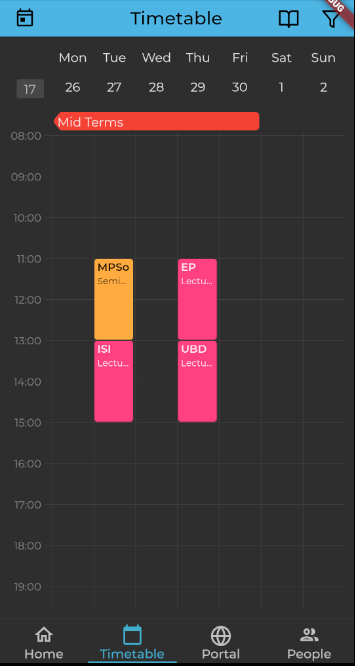
\includegraphics[width=0.5\columnwidth]{figures/c5/image21.png}
            \captionsetup{labelsep=space}
            \caption{Screenshot of the timetable}
            \label{5:fig:timetable}
        \end{wrapfigure}
	As we can see in figure \ref{5:fig:timetable}, taken directly from the application, we can split the view into three main zones of interest : 

	\begin{itemize}
            \setlength{\topsep}{0.5pt}
            \setlength{\itemsep}{0.5pt}
            \setlength{\parsep}{0.5pt}
            \item Date header
            \item All-day events bar
            \item Class events 
            
\end{itemize}


For our implementation, in which the tasks are all-day events, we will use the all-day events bar to display them. The main benefit is that it generates a simplified Gantt chart of the tasks the users have to complete, and it also visually distinguishes them from other types of events\footnote{https://github.com/JonasWanke/timetable}. 
	
Adding a task follows the same process of adding any other event, as it requires the user to preferably tap on the day in which the event starts, choose the corresponding type, and complete the other fields. Editing them works exactly like editing any other event. 
\clearpage
\section{Red Routes} \label{5:routes}

 We define the Red Routes as the critical functionalities that bring the most value for our users. To highlight them, we have to look at the usability matrix for all the proposed functionalities presented in figure \ref{5:fig:matrix}.
 
 
\begin{figure}[ht]
    \centering
         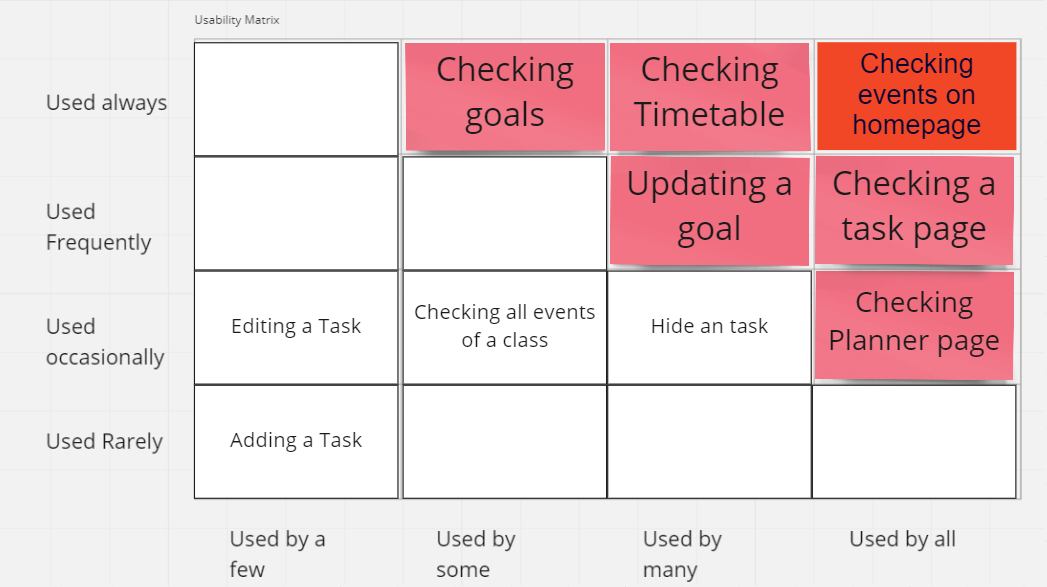
\includegraphics[width=0.95\textwidth]{figures/c5/image11.png}
    \caption{Red Routes matrix} 
    \label{5:fig:matrix}
\end{figure}


When making the matrix, we analyzed each functionality by two factors: the number of users and the frequency of being used. Presented in red background, those functionalities are critical for the purpose of optimizing the university schedule, as they are used by a majority of the users frequently. On the other hand, even though not very used, the functionalities in the lower part of the main diagonal are vital for the other features, as they deal with creating the events used by more user-centered features. 

As the figure indicates, the most important functionalities for the users are those that quickly give them information about events and tasks in the near future. This provides them with a better understanding of how time is partitioned and how it should be managed to accomplish everything that is tracked.

\section{Wireframes} \label{5:Wireframes}

As every visual update has to be coherent with the other components, we want to first conceptualize new elements by including them in new wireframes. By doing so, we can have a general view of how they should be positioned.
This way, we ensure that the user recognizes the new features and quickly understands and uses them. 

Based on the features that we want to add, we identified the pages that should contain them, and for those that need a new page, we choose the best way to integrate a new flow in the application:

\begin{figure}[!ht]
    \centering
    \begin{minipage}[b]{0.45\textwidth}
        \captionsetup{justification=centering}
        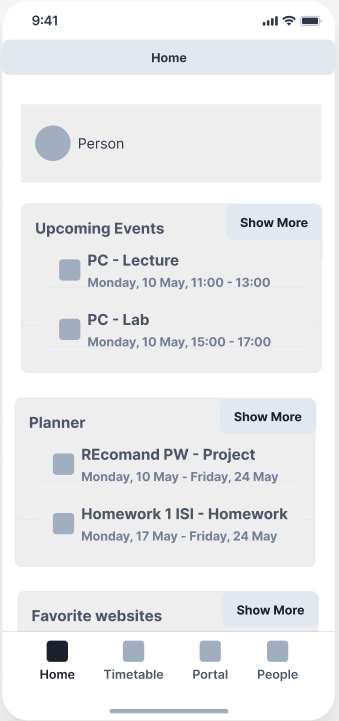
\includegraphics[width=\textwidth]{figures/wf/image15.png}
        \caption{Home page}
        \label{5:fig:homepage}
    \end{minipage}
    \hfill
    \begin{minipage}[b]{0.45\textwidth}
        \captionsetup{justification=centering}
        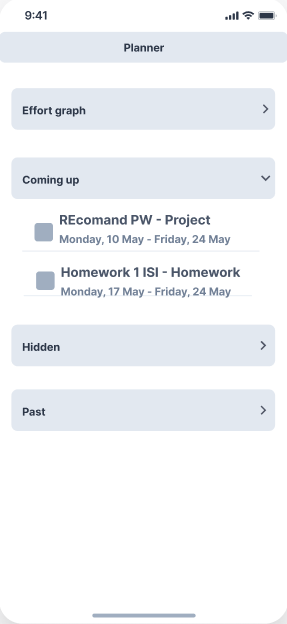
\includegraphics[width=\textwidth]{figures/wf/image7.png}
        \caption{Planner page}
        \label{5:fig:planner}
    \end{minipage}
    
\end{figure}
~
Homepage (figure \ref{5:fig:homepage}) has conceptually integrated within the new Cards. In Upcoming events we have a short list of upcoming class events. For each event, we show the class abbreviation, type, and time frame. The \textit{Show More} button redirects to the timetable.
The Planner card follows the same logic, showing for each element the name, class abbreviation, type, and the start and end date. The difference is \textit{Show More} redirects to the the Planner page (fig. \ref{5:fig:planner}).

The Planner has is divided in four sections. The first is reserved for the distribution graph of tasks throughout the semester. The others contain tasks that comply with the category suggested in the title. Tapping on the title shows or hides the list of containing items.
~
\begin{figure}[!ht]
    \centering
    \begin{minipage}[b]{0.43\textwidth}
        \captionsetup{justification=centering}
        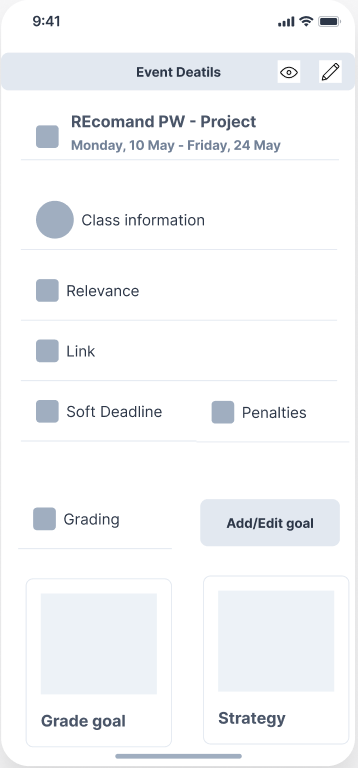
\includegraphics[width=\textwidth]{figures/wf/image51.png}
        \caption{Event Details page}
        \label{5:fig:eventdeatils}
    \end{minipage}
    \hfill
    \begin{minipage}[b]{0.43\textwidth}
        \captionsetup{justification=centering}
        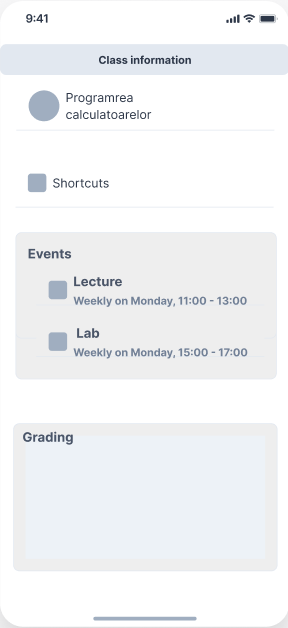
\includegraphics[width=\textwidth]{figures/wf/image17.png}
        \caption{Class Information page}
        \label{5:fig:classinfo}
    \end{minipage}
    
\end{figure}
\clearpage
Tapping on an task, it redirects to the event details page (figure \ref{5:fig:eventdeatils}). Here we have all the fields specific to tasks and also the goal button, and the visibility and edit button. For an event that already has set goals, like the one in the figure (figure \ref{5:fig:eventdeatils}), it also displays them in separate cards.

In the class information page (figure \ref{5:fig:classinfo}), we have added a new Card to display all it's all events in just one place.

~

\begin{figure}[!ht]
    \centering
    \begin{minipage}[b]{0.43\textwidth}
        \captionsetup{justification=centering}
        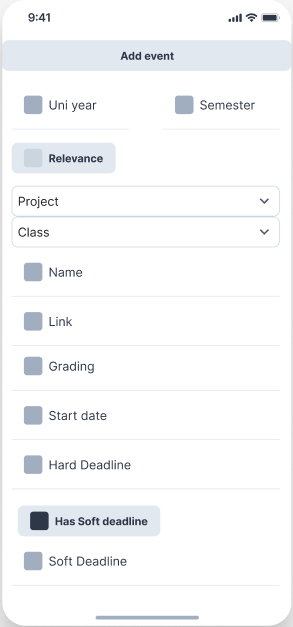
\includegraphics[width=\textwidth]{figures/wf/image3.png}
        \caption{Add/Edit event page}
        \label{5:fig:eventadd}
    \end{minipage}
    \hfill
    \begin{minipage}[b]{0.43\textwidth}
        \captionsetup{justification=centering}
        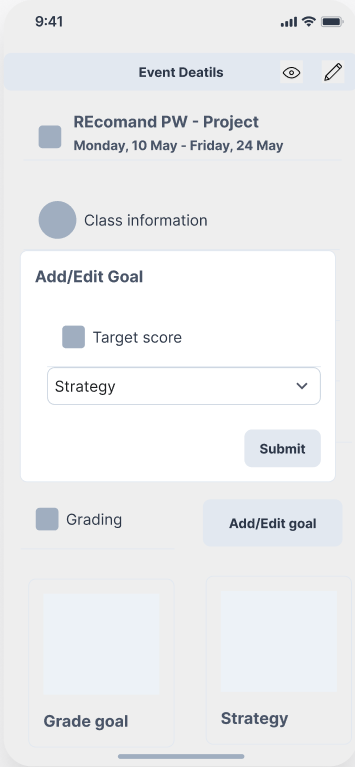
\includegraphics[width=\textwidth]{figures/wf/image52.png}
        \caption{Add/Edit goal}
        \label{5:fig:goalsadd}
    \end{minipage}
    
\end{figure}

~

In figures \ref{5:fig:eventadd} and \ref{5:fig:goalsadd}, we have the new form for adding or editing an task in a separate page, respectively an goal in a pop-up.


\section{Final UI} \label{5:finalui}

After we established the wireframes, we now will present the final implementation of Homepage (fig. \ref{5:fig:fhomepage}), Planner (fig. \ref{5:fig:fplanner}), Timetable (fig. \ref{5:fig:ftimetable}), Event Details page (fig. \ref{5:fig:fevent}), Class Information page (fig. \ref{5:fig:fclass}), Add/Edit event page (fig. \ref{5:fig:faddevent}), and Add/Edit goal pop-up (fig. \ref{5:fig:faddgoal}).

~

\begin{figure}[!ht]
    \centering
    \begin{minipage}[b]{0.32\textwidth}
        \captionsetup{justification=centering}
        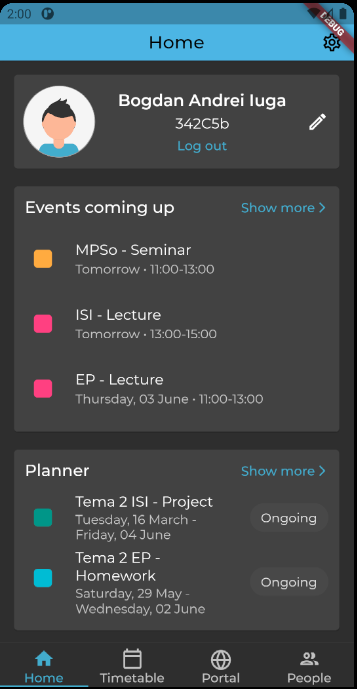
\includegraphics[width=\textwidth]{figures/ss/image7.png}
        \caption{Homepage}
        \label{5:fig:fhomepage}
    \end{minipage}
    \hfill
    \begin{minipage}[b]{0.32\textwidth}
        \captionsetup{justification=centering}
        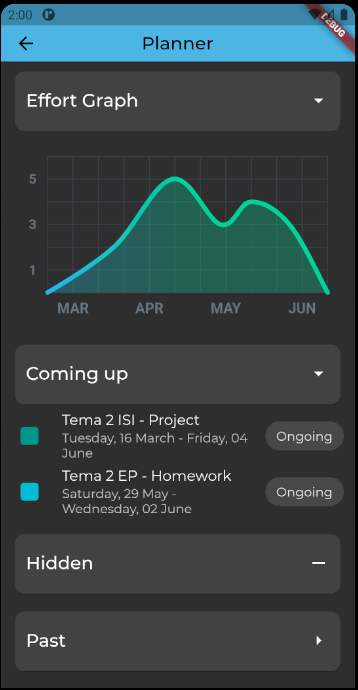
\includegraphics[width=\textwidth]{figures/ss/image3.png}
        \caption{Planner}
        \label{5:fig:fplanner}
    \end{minipage}
     \hfill
    \begin{minipage}[b]{0.32\textwidth}
        \captionsetup{justification=centering}
        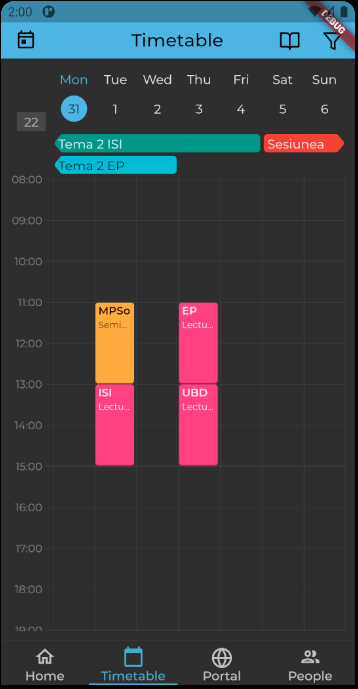
\includegraphics[width=\textwidth]{figures/ss/image2.png}
        \caption{Timetable}
        \label{5:fig:ftimetable}
    \end{minipage}
    
\end{figure}


\begin{figure}[!ht]
    \centering
    \begin{minipage}[b]{0.35\textwidth}
        \captionsetup{justification=centering}
        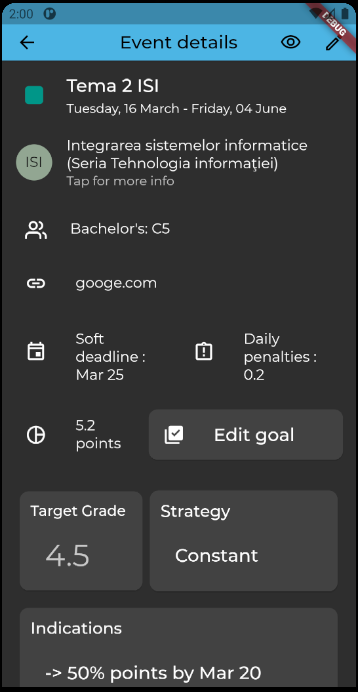
\includegraphics[width=\textwidth]{figures/ss/image5.png}
        \caption{Event page}
        \label{5:fig:fevent}
    \end{minipage}
    \hfill
    \begin{minipage}[b]{0.35\textwidth}
        \captionsetup{justification=centering}
        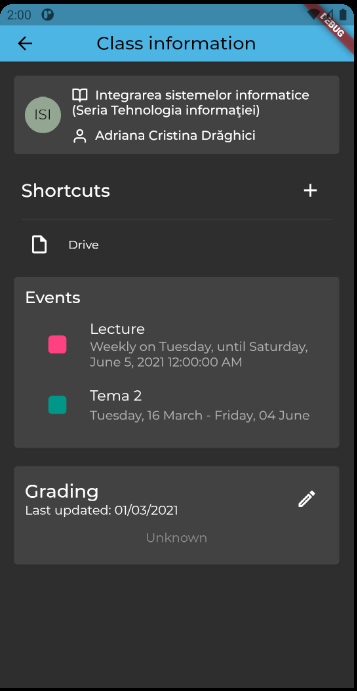
\includegraphics[width=\textwidth]{figures/ss/image4.png}
        \caption{Class page}
        \label{5:fig:fclass}
    \end{minipage}
    
\end{figure}

\begin{figure}[!ht]
    \centering
    \begin{minipage}[b]{0.35\textwidth}
        \captionsetup{justification=centering}
        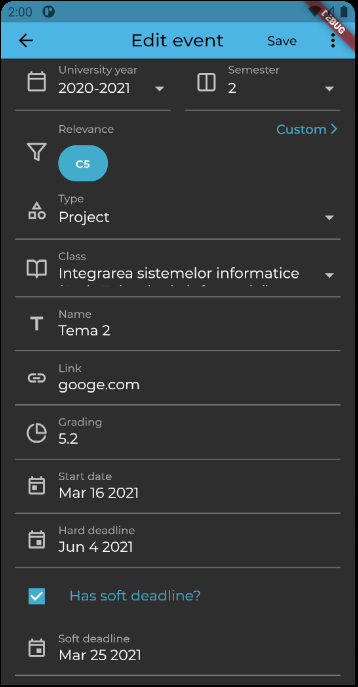
\includegraphics[width=\textwidth]{figures/ss/image6.png}
        \caption{Add/Edit event}
        \label{5:fig:faddevent}
    \end{minipage}
    \hfill
    \begin{minipage}[b]{0.35\textwidth}
        \captionsetup{justification=centering}
        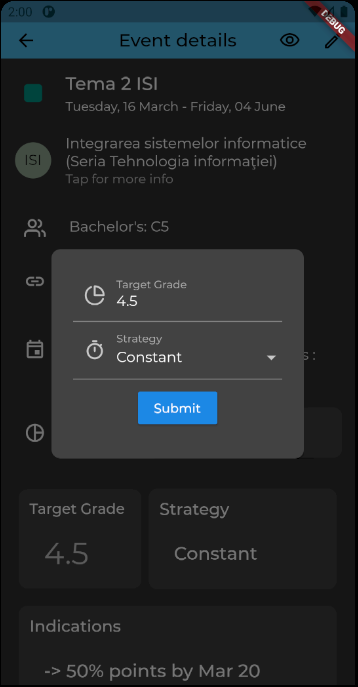
\includegraphics[width=\textwidth]{figures/ss/image1.png}
        \caption{Add/Edit goal}
        \label{5:fig:faddgoal}
    \end{minipage}
    
\end{figure}

~